\documentclass[aspectratio=169,11pt]{beamer}

% Compile with XeLaTeX
\usepackage{fontspec}
\setsansfont{DejaVu Sans}
\setmonofont{DejaVu Sans Mono}
\usepackage{polyglossia}
\setdefaultlanguage{vietnamese}
\usepackage{booktabs}
\usepackage{array}
\usepackage{tabularx}
\usepackage{listings}
\usepackage{xcolor}
\usepackage{ragged2e}

% Graphics
\usepackage{graphicx}
\graphicspath{{images/}}

\usetheme{Madrid}
\usecolortheme{seahorse}
\setbeamertemplate{navigation symbols}{}
\setbeamertemplate{footline}[frame number]
\setbeamertemplate{itemize items}[circle]
\setbeamertemplate{enumerate items}[default]

\definecolor{codebg}{RGB}{248,248,248}
\definecolor{codekw}{RGB}{0,72,160}
\definecolor{codestr}{RGB}{150,60,30}
\definecolor{accent}{RGB}{0,90,150}

\lstset{
  basicstyle=\ttfamily\scriptsize,
  keywordstyle=\color{codekw}\bfseries,
  stringstyle=\color{codestr},
  backgroundcolor=\color{codebg},
  frame=single,
  breaklines=true,
  columns=fullflexible,
  showstringspaces=false,
  keepspaces=true,
  language=SQL
}

\newcommand{\keyword}[1]{\textcolor{accent}{\textbf{#1}}}
\newcommand{\tightlist}{\setlength{\itemsep}{2pt}\setlength{\parskip}{0pt}}
\newcommand{\qoption}[2]{\item[#1.] #2}

\title[Giới thiệu về CSDL]{Giới thiệu về Cơ sở dữ liệu}
\subtitle{Database, DBMS, RDBMS, NoSQL và ACID}
\author{Tài liệu bài giảng}
\institute{Môn học: Cơ sở dữ liệu}
\date{Cập nhật: 28/04/2026}

\begin{document}

%------------------------------------------------
\begin{frame}
  \titlepage
\end{frame}

%------------------------------------------------
\begin{frame}{Mục tiêu bài giảng}
\small
Sau bài học này, người học có thể:
\begin{enumerate}
\tightlist
  \item Giải thích khái niệm \keyword{dữ liệu} và \keyword{cơ sở dữ liệu}.
  \item Trình bày vai trò của \keyword{DBMS} trong lưu trữ, truy xuất và quản lý dữ liệu.
  \item Mô tả các thành phần chính của một cơ sở dữ liệu.
  \item Phân biệt \keyword{Relational Database} và \keyword{NoSQL Database}.
  \item Giải thích ý nghĩa của các tính chất \keyword{ACID}.
  \item Nhận diện ứng dụng thực tế của cơ sở dữ liệu trong nhiều lĩnh vực.
  \item Lựa chọn loại cơ sở dữ liệu phù hợp cho một số miền công nghệ.
\end{enumerate}
\end{frame}

%------------------------------------------------
\begin{frame}{Dữ liệu và thông tin}
\small
\begin{block}{Dữ liệu}
Dữ liệu là các sự kiện, con số hoặc thông tin thô, chưa được tổ chức và chưa có nhiều ý nghĩa nếu đứng riêng lẻ.
\end{block}

\begin{columns}[T]
\column{0.48\textwidth}
Ví dụ dữ liệu:
\begin{itemize}
\tightlist
  \item Tên khách hàng
  \item Số điện thoại
  \item Mã sinh viên
  \item Điểm thi
  \item Ngày giao dịch
  \item Ảnh, video, âm thanh
\end{itemize}

\column{0.48\textwidth}
\begin{block}{Thông tin}
Khi dữ liệu được xử lý, sắp xếp và phân tích, nó tạo ra thông tin có ý nghĩa phục vụ ra quyết định.
\end{block}
\end{columns}
\end{frame}

%------------------------------------------------
\begin{frame}{Cơ sở dữ liệu là gì?}
\small
\begin{block}{Định nghĩa}
Cơ sở dữ liệu là một hệ thống có cấu trúc dùng để \textbf{lưu trữ}, \textbf{quản lý}, \textbf{truy xuất} và \textbf{cập nhật} dữ liệu một cách hiệu quả cho nhiều người dùng và nhiều ứng dụng.
\end{block}

Cơ sở dữ liệu quan trọng vì:
\begin{itemize}
\tightlist
  \item \keyword{Scalability}: xử lý khối lượng dữ liệu lớn.
  \item \keyword{Data Integrity}: duy trì độ chính xác bằng quy tắc và ràng buộc.
  \item \keyword{Security}: bảo vệ dữ liệu bằng quyền truy cập và phân quyền.
  \item \keyword{Analytics}: hỗ trợ phân tích và ra quyết định.
\end{itemize}
\end{frame}

\begin{frame}{Minh họa: Vì sao cơ sở dữ liệu quan trọng}
\centering
\vfill
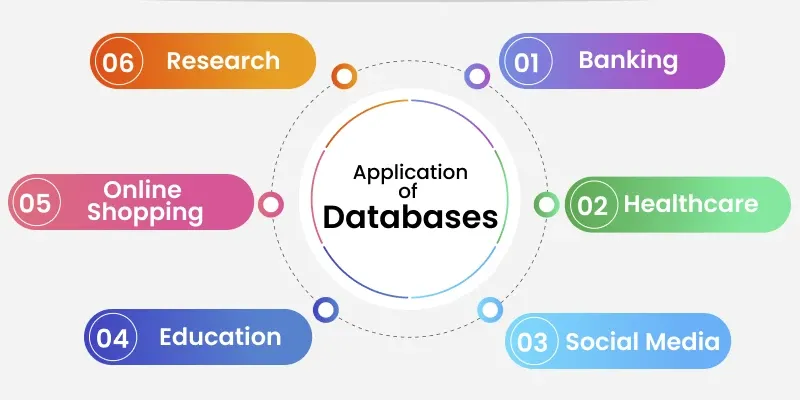
\includegraphics[width=0.78\textwidth,height=0.68\textheight,keepaspectratio]{image-4.png}
\vfill
\end{frame}

%------------------------------------------------
\begin{frame}{Quiz: Khái niệm dữ liệu và cơ sở dữ liệu}
\small
\textbf{Câu 1.} Dữ liệu là gì?
\begin{enumerate}
\tightlist
  \qoption{A}{Thông tin đã được phân tích hoàn chỉnh}
  \qoption{B}{Các sự kiện, con số hoặc thông tin thô chưa được xử lý}
  \qoption{C}{Một phần mềm quản lý dữ liệu}
  \qoption{D}{Một dạng ngôn ngữ lập trình}
\end{enumerate}

\textbf{Câu 2.} Cơ sở dữ liệu được dùng chủ yếu để làm gì?
\begin{enumerate}
\tightlist
  \qoption{A}{Thiết kế giao diện người dùng}
  \qoption{B}{Lưu trữ, quản lý và truy xuất dữ liệu}
  \qoption{C}{Chỉ để viết chương trình Python}
  \qoption{D}{Chỉ để lưu ảnh}
\end{enumerate}
\end{frame}

%------------------------------------------------
\begin{frame}{Quiz: Khái niệm dữ liệu và cơ sở dữ liệu (tiếp)}
\small
\textbf{Câu 3.} Đặc điểm nào giúp cơ sở dữ liệu xử lý khối lượng dữ liệu lớn?
\begin{enumerate}
\tightlist
  \qoption{A}{Security}
  \qoption{B}{Scalability}
  \qoption{C}{Isolation}
  \qoption{D}{Durability}
\end{enumerate}
\end{frame}

%------------------------------------------------
\begin{frame}{Cách cơ sở dữ liệu hoạt động}
\small
Cơ sở dữ liệu tổ chức và lưu trữ thông tin theo dạng có cấu trúc hoặc phi cấu trúc, cho phép người dùng dễ dàng:
\begin{itemize}
\tightlist
  \item Truy cập, tìm kiếm và truy xuất dữ liệu.
  \item Cập nhật, xóa và quản lý dữ liệu.
  \item Quản lý quyền truy cập.
\end{itemize}

\begin{block}{Vai trò trung tâm của DBMS}
DBMS là lớp phần mềm trung gian giữa người dùng và dữ liệu thô. Người dùng tương tác với DBMS thông qua câu lệnh truy vấn hoặc ứng dụng, thay vì làm việc trực tiếp với chi tiết lưu trữ vật lý.
\end{block}
\end{frame}

%------------------------------------------------
\begin{frame}{Quy trình xử lý yêu cầu trong DBMS}
\small
\begin{enumerate}
\tightlist
  \item Người dùng hoặc ứng dụng gửi yêu cầu đến DBMS.
  \item DBMS kiểm tra cú pháp, quyền truy cập và tối ưu hóa truy vấn.
  \item DBMS truy cập dữ liệu liên quan từ bảng, chỉ mục hoặc tệp lưu trữ.
  \item DBMS trả kết quả về cho người dùng hoặc ứng dụng.
\end{enumerate}

\vspace{0.2cm}
DBMS còn cung cấp:
\begin{itemize}
\tightlist
  \item Sao lưu và khôi phục dữ liệu.
  \item Tối ưu hiệu năng.
  \item Quản lý giao dịch.
  \item Kiểm soát truy cập.
  \item Quản lý đồng thời nhiều người dùng.
\end{itemize}
\end{frame}

\begin{frame}{Minh họa: Quy trình xử lý yêu cầu trong DBMS}
\centering
\vfill
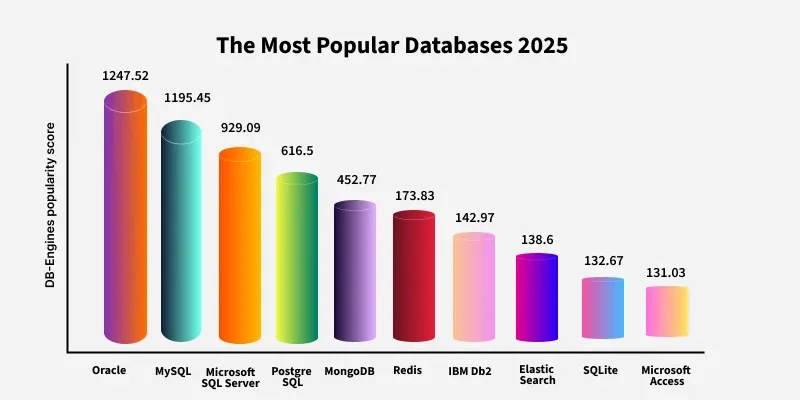
\includegraphics[width=0.80\textwidth,height=0.66\textheight,keepaspectratio]{image-5.png}
\vfill
\end{frame}

%------------------------------------------------
\begin{frame}{Quiz: Cách cơ sở dữ liệu hoạt động}
\small
\textbf{Câu 1.} DBMS đóng vai trò gì trong hệ thống cơ sở dữ liệu?
\begin{enumerate}
\tightlist
  \qoption{A}{Là lớp trung gian giữa người dùng và dữ liệu}
  \qoption{B}{Là thiết bị phần cứng dùng để lưu trữ dữ liệu}
  \qoption{C}{Là ngôn ngữ lập trình thay thế SQL}
  \qoption{D}{Là phần mềm chỉ dùng để vẽ biểu đồ}
\end{enumerate}

\textbf{Câu 2.} Khi người dùng gửi truy vấn, DBMS thường làm gì?
\begin{enumerate}
\tightlist
  \qoption{A}{Bỏ qua truy vấn}
  \qoption{B}{Xử lý truy vấn, tìm dữ liệu phù hợp và trả kết quả}
  \qoption{C}{Luôn xóa dữ liệu trước khi trả kết quả}
  \qoption{D}{Chỉ lưu truy vấn vào tệp văn bản}
\end{enumerate}
\end{frame}

%------------------------------------------------
\begin{frame}{Quiz: Cách cơ sở dữ liệu hoạt động (tiếp)}
\small
\textbf{Câu 3.} Chức năng nào sau đây là chức năng quan trọng của DBMS?
\begin{enumerate}
\tightlist
  \qoption{A}{Sao lưu và khôi phục dữ liệu}
  \qoption{B}{Chỉ phát nhạc}
  \qoption{C}{Chỉ chỉnh sửa ảnh}
  \qoption{D}{Chỉ biên dịch chương trình C++}
\end{enumerate}
\end{frame}

%------------------------------------------------

\begin{frame}{Các thành phần của một cơ sở dữ liệu}
\small
Một cơ sở dữ liệu bao gồm nhiều thành phần phối hợp với nhau để lưu trữ, tổ chức, quản lý và truy xuất dữ liệu hiệu quả.

\vspace{0.25cm}
\begin{tabularx}{\textwidth}{>{\bfseries}p{0.24\textwidth} X}
\toprule
Thành phần & Vai trò chính \\
\midrule
Dữ liệu & Thông tin thực tế được lưu trong cơ sở dữ liệu. \\
Schema & Bản thiết kế mô tả cách dữ liệu được tổ chức. \\
DBMS & Phần mềm quản lý các hoạt động của cơ sở dữ liệu. \\
Query & Chỉ dẫn dùng để lấy, thêm, cập nhật hoặc xóa dữ liệu. \\
Người dùng & Cá nhân hoặc hệ thống tương tác với cơ sở dữ liệu. \\
\bottomrule
\end{tabularx}
\end{frame}

\begin{frame}{Minh họa: Thành phần cơ sở dữ liệu}
\centering
\vfill
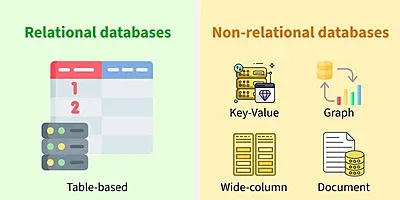
\includegraphics[width=0.84\textwidth,height=0.62\textheight,keepaspectratio]{image-6.png}
\vfill
\end{frame}

%------------------------------------------------
\begin{frame}{Thành phần 1: Dữ liệu}
\small
\begin{block}{Khái niệm}
\keyword{Dữ liệu} là thông tin thực tế được lưu trong cơ sở dữ liệu.
\end{block}

Dữ liệu có thể là:
\begin{itemize}
\tightlist
  \item Văn bản, số, ngày tháng.
  \item Hình ảnh, tệp tin, âm thanh, video.
  \item Dữ liệu cảm biến hoặc dữ liệu sinh ra từ hệ thống.
\end{itemize}

\begin{exampleblock}{Ví dụ}
Trong hệ thống quản lý sinh viên, dữ liệu có thể gồm mã sinh viên, họ tên, ngày sinh, lớp, điểm thi và trạng thái học tập.
\end{exampleblock}
\end{frame}

%------------------------------------------------
\begin{frame}{Thành phần 2: Lược đồ cơ sở dữ liệu}
\small
\begin{block}{Schema}
\keyword{Schema} hay \keyword{lược đồ cơ sở dữ liệu} là bản thiết kế mô tả cách dữ liệu được tổ chức.
\end{block}

Lược đồ có thể mô tả:
\begin{itemize}
\tightlist
  \item Các bảng và các trường dữ liệu.
  \item Kiểu dữ liệu của từng trường.
  \item Khóa chính và khóa ngoại.
  \item Quan hệ giữa các bảng.
  \item Các ràng buộc dữ liệu.
\end{itemize}
\end{frame}

%------------------------------------------------
\begin{frame}{Ví dụ về lược đồ cơ sở dữ liệu}
\small
Trong cơ sở dữ liệu quản lý bán hàng, lược đồ có thể gồm các bảng:

\begin{itemize}
\tightlist
  \item \texttt{Customers}: lưu thông tin khách hàng.
  \item \texttt{Orders}: lưu thông tin đơn hàng.
  \item \texttt{Products}: lưu thông tin sản phẩm.
  \item \texttt{OrderDetails}: lưu chi tiết từng dòng sản phẩm trong đơn hàng.
\end{itemize}

\begin{block}{Ý nghĩa}
Schema giúp hệ thống biết dữ liệu được tổ chức như thế nào, các bảng liên kết ra sao và dữ liệu cần tuân thủ những ràng buộc nào.
\end{block}
\end{frame}

%------------------------------------------------
\begin{frame}{Thành phần 3: Hệ quản trị cơ sở dữ liệu}
\small
\begin{block}{DBMS}
\keyword{DBMS} là phần mềm quản lý các hoạt động của cơ sở dữ liệu.
\end{block}

DBMS hỗ trợ các chức năng như:
\begin{itemize}
\tightlist
  \item Lưu trữ, truy xuất, cập nhật và xóa dữ liệu.
  \item Quản lý bảo mật và người dùng.
  \item Quản lý giao dịch.
  \item Sao lưu và khôi phục dữ liệu.
\end{itemize}
\end{frame}

%------------------------------------------------
\begin{frame}{Ví dụ về DBMS}
\small
Một số hệ quản trị cơ sở dữ liệu phổ biến:

\begin{columns}[T]
\column{0.5\textwidth}
\begin{itemize}
\tightlist
  \item MySQL.
  \item PostgreSQL.
  \item Oracle.
\end{itemize}

\column{0.5\textwidth}
\begin{itemize}
\tightlist
  \item Microsoft SQL Server.
  \item MongoDB.
\end{itemize}
\end{columns}

\vspace{0.25cm}
\begin{block}{Ghi nhớ}
DBMS không chỉ lưu dữ liệu mà còn kiểm soát cách dữ liệu được truy cập, bảo vệ, cập nhật và phục hồi khi có sự cố.
\end{block}
\end{frame}

\begin{frame}{Minh họa: Hệ quản trị cơ sở dữ liệu}
\centering
\vfill
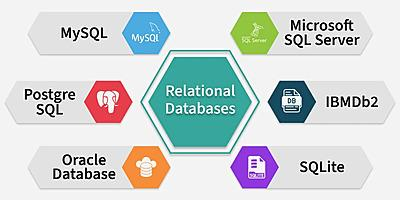
\includegraphics[width=0.84\textwidth,height=0.62\textheight,keepaspectratio]{image-7.png}
\vfill
\end{frame}

%------------------------------------------------
\begin{frame}[fragile]{Thành phần 4: Truy vấn}
\small
\begin{block}{Query}
\keyword{Query} hay \keyword{truy vấn} là chỉ dẫn dùng để lấy, thêm, cập nhật hoặc xóa dữ liệu trong cơ sở dữ liệu.
\end{block}

Trong cơ sở dữ liệu quan hệ, truy vấn thường được viết bằng \keyword{SQL}.

\begin{lstlisting}
SELECT * FROM Students
WHERE major = 'Data Science';
\end{lstlisting}

Truy vấn trên dùng để lấy danh sách sinh viên thuộc ngành \textit{Data Science}.
\end{frame}

%------------------------------------------------
\begin{frame}{Thành phần 5: Người dùng}
\small
Người dùng là những cá nhân hoặc hệ thống tương tác với cơ sở dữ liệu.

\vspace{0.15cm}
Một số nhóm người dùng phổ biến:
\begin{itemize}
\tightlist
  \item Quản trị viên cơ sở dữ liệu.
  \item Lập trình viên.
  \item Nhà phân tích dữ liệu.
  \item Người dùng cuối.
  \item Ứng dụng phần mềm.
  \item Hệ thống tự động.
\end{itemize}

\begin{block}{Phân quyền}
Mỗi nhóm người dùng có thể có quyền truy cập khác nhau tùy theo vai trò.
\end{block}
\end{frame}

%------------------------------------------------
\begin{frame}{Hai nhóm cơ sở dữ liệu phổ biến}
\small
\begin{columns}[T]
\column{0.48\textwidth}
\begin{block}{Relational Database}
\begin{itemize}
\tightlist
  \item Tổ chức dữ liệu thành bảng.
  \item Có hàng, cột, khóa chính, khóa ngoại.
  \item Dùng SQL phổ biến.
  \item Phù hợp dữ liệu có cấu trúc.
\end{itemize}
\end{block}

\column{0.48\textwidth}
\begin{block}{NoSQL Database}
\begin{itemize}
\tightlist
  \item Linh hoạt hơn về mô hình dữ liệu.
  \item Phù hợp dữ liệu phi cấu trúc hoặc bán cấu trúc.
  \item Hỗ trợ mở rộng ngang tốt.
  \item Gồm document, key-value, wide-column, graph.
\end{itemize}
\end{block}
\end{columns}
\end{frame}

%------------------------------------------------
\begin{frame}{Cơ sở dữ liệu quan hệ}
\small
\keyword{Relational Database} tổ chức dữ liệu thành các bảng. Mỗi bảng gồm:
\begin{itemize}
\tightlist
  \item \textbf{Rows/Records}: các bản ghi cụ thể.
  \item \textbf{Columns/Fields}: các thuộc tính của bản ghi.
\end{itemize}

\begin{table}[]
\centering
\scriptsize
\begin{tabular}{llll}
\toprule
StudentID & FullName & Major & GPA \\
\midrule
S001 & Nguyễn An & Data Science & 3.4 \\
S002 & Trần Bình & AI & 3.7 \\
S003 & Lê Chi & Information Systems & 3.2 \\
\bottomrule
\end{tabular}
\end{table}
\end{frame}

%------------------------------------------------
\begin{frame}{Đặc điểm của cơ sở dữ liệu quan hệ}
\small
\begin{itemize}
\tightlist
  \item \textbf{Schema chặt chẽ}: bảng, cột, kiểu dữ liệu và ràng buộc được định nghĩa trước.
  \item \textbf{Primary key}: định danh duy nhất mỗi bản ghi trong bảng.
  \item \textbf{Foreign key}: biểu diễn quan hệ giữa các bảng.
  \item \textbf{ACID}: đảm bảo giao dịch đáng tin cậy.
  \item \textbf{Dữ liệu có cấu trúc}: phù hợp với kế toán, ngân hàng, sinh viên, bán hàng.
\end{itemize}

Ví dụ RDBMS: MySQL, PostgreSQL, Oracle, Microsoft SQL Server.
\end{frame}

%------------------------------------------------
\begin{frame}{Quiz: Cơ sở dữ liệu quan hệ}
\small
\textbf{Câu 1.} Cơ sở dữ liệu quan hệ tổ chức dữ liệu chủ yếu dưới dạng nào?
\begin{enumerate}
\tightlist
  \qoption{A}{Đồ thị}
  \qoption{B}{Bảng gồm hàng và cột}
  \qoption{C}{Tệp âm thanh}
  \qoption{D}{Chuỗi khối}
\end{enumerate}

\textbf{Câu 2.} Primary key dùng để làm gì?
\begin{enumerate}
\tightlist
  \qoption{A}{Định danh duy nhất mỗi bản ghi trong bảng}
  \qoption{B}{Xóa toàn bộ cơ sở dữ liệu}
  \qoption{C}{Mã hóa hình ảnh}
  \qoption{D}{Tạo giao diện người dùng}
\end{enumerate}
\end{frame}

%------------------------------------------------
\begin{frame}{Quiz: Cơ sở dữ liệu quan hệ (tiếp)}
\small
\textbf{Câu 3.} Ví dụ nào sau đây là RDBMS?
\begin{enumerate}
\tightlist
  \qoption{A}{PostgreSQL}
  \qoption{B}{Redis}
  \qoption{C}{Neo4j}
  \qoption{D}{IPFS}
\end{enumerate}
\end{frame}

%------------------------------------------------
\begin{frame}{Cơ sở dữ liệu NoSQL}
\small
\keyword{NoSQL} là viết tắt của \textit{Not Only SQL}. NoSQL được thiết kế để xử lý dữ liệu phi cấu trúc hoặc bán cấu trúc như:
\begin{itemize}
\tightlist
  \item Văn bản, hình ảnh, video.
  \item Dữ liệu cảm biến.
  \item Log hệ thống.
  \item Dữ liệu mạng xã hội.
  \item Dữ liệu thời gian thực.
\end{itemize}

Khác với RDBMS, NoSQL không nhất thiết lưu dữ liệu dưới dạng bảng cố định.
\end{frame}

%------------------------------------------------
\begin{frame}{Các loại NoSQL chính}
\small
\begin{tabularx}{\textwidth}{>{\bfseries}p{0.24\textwidth} X p{0.22\textwidth}}
\toprule
Loại & Mô tả & Ví dụ \\
\midrule
Document & Lưu dữ liệu dạng tài liệu giống JSON & MongoDB \\
Key-value & Lưu cặp khóa - giá trị, tra cứu nhanh & Redis \\
Wide-column & Lưu dữ liệu theo cột, phù hợp big data & Cassandra \\
Graph & Lưu nút và quan hệ giữa các nút & Neo4j \\
\bottomrule
\end{tabularx}
\end{frame}

%------------------------------------------------
\begin{frame}{Quiz: Cơ sở dữ liệu NoSQL}
\small
\textbf{Câu 1.} NoSQL là viết tắt của cụm từ nào?
\begin{enumerate}
\tightlist
  \qoption{A}{No Software Query Language}
  \qoption{B}{Not Only SQL}
  \qoption{C}{New Online SQL}
  \qoption{D}{Normal SQL}
\end{enumerate}

\textbf{Câu 2.} Loại NoSQL nào lưu dữ liệu dưới dạng cặp khóa - giá trị?
\begin{enumerate}
\tightlist
  \qoption{A}{Document database}
  \qoption{B}{Key-value store}
  \qoption{C}{Graph database}
  \qoption{D}{Relational database}
\end{enumerate}
\end{frame}

%------------------------------------------------
\begin{frame}{Quiz: Cơ sở dữ liệu NoSQL (tiếp)}
\small
\textbf{Câu 3.} Neo4j là ví dụ của loại cơ sở dữ liệu nào?
\begin{enumerate}
\tightlist
  \qoption{A}{Graph database}
  \qoption{B}{Key-value store}
  \qoption{C}{RDBMS}
  \qoption{D}{File system}
\end{enumerate}
\end{frame}

%------------------------------------------------
\begin{frame}{ACID là gì?}
\small
\keyword{ACID} gồm bốn tính chất quan trọng giúp giao dịch cơ sở dữ liệu đáng tin cậy, chính xác và an toàn.

\begin{tabularx}{\textwidth}{>{\bfseries}p{0.22\textwidth} X}
\toprule
Tính chất & Ý nghĩa \\
\midrule
Atomicity & Giao dịch phải được thực hiện toàn bộ hoặc không thực hiện gì cả. \\
Consistency & CSDL chuyển từ trạng thái hợp lệ sang trạng thái hợp lệ khác. \\
Isolation & Nhiều giao dịch đồng thời không gây ảnh hưởng sai lệch cho nhau. \\
Durability & Sau khi giao dịch hoàn tất, thay đổi được lưu bền vững. \\
\bottomrule
\end{tabularx}
\end{frame}

%------------------------------------------------
\begin{frame}{Ví dụ ACID: chuyển tiền ngân hàng}
\small
Khi chuyển tiền từ tài khoản A sang tài khoản B:
\begin{enumerate}
\tightlist
  \item Trừ tiền tài khoản A.
  \item Cộng tiền vào tài khoản B.
\end{enumerate}

\begin{itemize}
\tightlist
  \item \textbf{Atomicity}: nếu bước 2 thất bại, bước 1 phải bị hủy.
  \item \textbf{Consistency}: số dư sau giao dịch vẫn hợp lệ.
  \item \textbf{Isolation}: giao dịch đồng thời không làm sai lệch dữ liệu.
  \item \textbf{Durability}: giao dịch thành công phải được lưu bền vững.
\end{itemize}
\end{frame}

%------------------------------------------------
\begin{frame}{Quiz: Tính chất ACID}
\small
\textbf{Câu 1.} ACID gồm những tính chất nào?
\begin{enumerate}
\tightlist
  \qoption{A}{Accuracy, Control, Integrity, Design}
  \qoption{B}{Atomicity, Consistency, Isolation, Durability}
  \qoption{C}{Access, Cache, Index, Data}
  \qoption{D}{Application, Cloud, Internet, Database}
\end{enumerate}

\textbf{Câu 2.} Tính chất nào đảm bảo giao dịch được thực hiện toàn bộ hoặc không thực hiện gì cả?
\begin{enumerate}
\tightlist
  \qoption{A}{Atomicity}
  \qoption{B}{Consistency}
  \qoption{C}{Isolation}
  \qoption{D}{Durability}
\end{enumerate}
\end{frame}

%------------------------------------------------
\begin{frame}{Quiz: Tính chất ACID (tiếp)}
\small
\textbf{Câu 3.} Tính chất nào đảm bảo dữ liệu vẫn được lưu sau khi giao dịch đã hoàn tất?
\begin{enumerate}
\tightlist
  \qoption{A}{Atomicity}
  \qoption{B}{Consistency}
  \qoption{C}{Isolation}
  \qoption{D}{Durability}
\end{enumerate}
\end{frame}

%------------------------------------------------
\begin{frame}{Ứng dụng thực tế của cơ sở dữ liệu}
\small
\begin{tabularx}{\textwidth}{>{\bfseries}p{0.23\textwidth} X}
\toprule
Lĩnh vực & Dữ liệu thường được quản lý \\
\midrule
Ngân hàng & Giao dịch, tài khoản, khoản vay, thông tin khách hàng. \\
Giao thông & Đặt vé, lịch trình, tuyến đường, phương tiện, hành khách. \\
Giáo dục & Hồ sơ sinh viên, điểm số, lịch học, học phí. \\
Bán lẻ & Tồn kho, đơn hàng, khách hàng, khuyến mãi, doanh thu. \\
Mạng xã hội & Người dùng, bài đăng, tin nhắn, ảnh, video, tương tác. \\
\bottomrule
\end{tabularx}
\end{frame}

%------------------------------------------------
\begin{frame}{Quiz: Ứng dụng cơ sở dữ liệu}
\small
\textbf{Câu 1.} Trong ngân hàng, cơ sở dữ liệu thường dùng để lưu gì?
\begin{enumerate}
\tightlist
  \qoption{A}{Giao dịch và tài khoản}
  \qoption{B}{Chỉ hình nền máy tính}
  \qoption{C}{Chỉ mã nguồn chương trình}
  \qoption{D}{Chỉ tệp âm thanh}
\end{enumerate}

\textbf{Câu 2.} Trong giáo dục, cơ sở dữ liệu có thể dùng để quản lý gì?
\begin{enumerate}
\tightlist
  \qoption{A}{Hồ sơ sinh viên và điểm số}
  \qoption{B}{Tốc độ quạt máy tính}
  \qoption{C}{Tín hiệu điều khiển tivi}
  \qoption{D}{Màu sắc giao diện}
\end{enumerate}
\end{frame}

%------------------------------------------------
\begin{frame}{Quiz: Ứng dụng cơ sở dữ liệu (tiếp)}
\small
\textbf{Câu 3.} Trong bán lẻ, cơ sở dữ liệu có thể hỗ trợ quản lý gì?
\begin{enumerate}
\tightlist
  \qoption{A}{Tồn kho và đơn hàng}
  \qoption{B}{Chỉ video cá nhân}
  \qoption{C}{Chỉ địa chỉ IP router}
  \qoption{D}{Chỉ trình phát nhạc}
\end{enumerate}
\end{frame}

%------------------------------------------------
\begin{frame}{Cơ sở dữ liệu trong các lĩnh vực công nghệ}
\small
\begin{itemize}
\tightlist
  \item \textbf{Web Development}: MySQL, PostgreSQL, MongoDB, Firebase.
  \item \textbf{Mobile Development}: SQLite, Realm, Firebase Realtime Database.
  \item \textbf{DevOps}: PostgreSQL, Redis, InfluxDB, Cassandra.
  \item \textbf{Data Engineering}: HDFS, Cassandra, Redshift, BigQuery.
  \item \textbf{Data Science}: PostgreSQL, MongoDB, Hive, Snowflake.
  \item \textbf{AI}: MongoDB, Cassandra, BigQuery, AWS S3.
  \item \textbf{Cloud}: Aurora, Cloud Spanner, Azure Cosmos DB.
  \item \textbf{Blockchain/Web3}: BigchainDB, IPFS, Ethereum, Chainlink.
\end{itemize}
\end{frame}

%------------------------------------------------
\begin{frame}{Quiz: Cơ sở dữ liệu theo lĩnh vực công nghệ}
\small
\textbf{Câu 1.} Cơ sở dữ liệu nào thường được dùng trong ứng dụng di động vì nhẹ và phù hợp lưu trữ cục bộ?
\begin{enumerate}
\tightlist
  \qoption{A}{SQLite}
  \qoption{B}{Oracle RAC}
  \qoption{C}{HDFS}
  \qoption{D}{Ethereum}
\end{enumerate}

\textbf{Câu 2.} Google BigQuery thường phù hợp với lĩnh vực nào?
\begin{enumerate}
\tightlist
  \qoption{A}{Data Engineering và phân tích dữ liệu lớn}
  \qoption{B}{Chỉ chỉnh sửa ảnh}
  \qoption{C}{Lập trình game offline nhỏ}
  \qoption{D}{Điều khiển bàn phím}
\end{enumerate}
\end{frame}

%------------------------------------------------
\begin{frame}{Quiz: Cơ sở dữ liệu theo lĩnh vực công nghệ (tiếp)}
\small
\textbf{Câu 3.} IPFS thường liên quan đến lĩnh vực nào?
\begin{enumerate}
\tightlist
  \qoption{A}{Blockchain/Web3}
  \qoption{B}{Quản lý lớp học truyền thống}
  \qoption{C}{Chỉ ứng dụng desktop cá nhân}
  \qoption{D}{Hệ điều hành Windows}
\end{enumerate}
\end{frame}

%------------------------------------------------
\begin{frame}{So sánh Relational Database và NoSQL}
\scriptsize
\begin{tabularx}{\textwidth}{>{\bfseries}p{0.20\textwidth} X X}
\toprule
Tiêu chí & Relational Database & NoSQL Database \\
\midrule
Cấu trúc & Bảng, hàng, cột & Tài liệu, key-value, cột rộng, đồ thị \\
Lược đồ & Thường cố định và chặt chẽ & Linh hoạt hơn \\
Ngôn ngữ & SQL & Tùy hệ quản trị \\
Quan hệ & Khóa chính, khóa ngoại, join & Tùy mô hình dữ liệu \\
Mở rộng & Thường mạnh về mở rộng dọc & Thường mạnh về mở rộng ngang \\
Phù hợp & Dữ liệu có cấu trúc & Dữ liệu phi cấu trúc/bán cấu trúc \\
Ví dụ & MySQL, PostgreSQL, Oracle & MongoDB, Redis, Cassandra, Neo4j \\
\bottomrule
\end{tabularx}
\end{frame}

%------------------------------------------------
\begin{frame}{Câu hỏi ôn tập: trắc nghiệm}
\small
\textbf{Câu 1.} Cơ sở dữ liệu là gì?
\begin{enumerate}
\tightlist
  \qoption{A}{Một hệ thống dùng để lưu trữ, quản lý và truy xuất dữ liệu}
  \qoption{B}{Một trình duyệt web}
  \qoption{C}{Một hệ điều hành}
  \qoption{D}{Một thiết bị nhập liệu}
\end{enumerate}

\textbf{Câu 2.} DBMS là gì?
\begin{enumerate}
\tightlist
  \qoption{A}{Phần mềm quản lý cơ sở dữ liệu}
  \qoption{B}{Một loại màn hình}
  \qoption{C}{Một giao thức mạng xã hội}
  \qoption{D}{Một phần mềm chỉ dùng để vẽ ảnh}
\end{enumerate}
\end{frame}

%------------------------------------------------
\begin{frame}{Câu hỏi ôn tập: trắc nghiệm (tiếp)}
\small
\textbf{Câu 3.} Thành phần nào mô tả cấu trúc bảng, trường và quan hệ?
\begin{enumerate}
\tightlist
  \qoption{A}{Schema}
  \qoption{B}{User}
  \qoption{C}{Query}
  \qoption{D}{File ảnh}
\end{enumerate}

\textbf{Câu 4.} Cơ sở dữ liệu quan hệ tổ chức dữ liệu thành gì?
\begin{enumerate}
\tightlist
  \qoption{A}{Bảng}
  \qoption{B}{Video}
  \qoption{C}{Tin nhắn thoại}
  \qoption{D}{Chuỗi bit ngẫu nhiên không có cấu trúc}
\end{enumerate}
\end{frame}

%------------------------------------------------
\begin{frame}{Câu hỏi ôn tập: trắc nghiệm (tiếp)}
\small
\textbf{Câu 5.} NoSQL phù hợp với loại dữ liệu nào?
\begin{enumerate}
\tightlist
  \qoption{A}{Phi cấu trúc hoặc bán cấu trúc}
  \qoption{B}{Chỉ dữ liệu dạng bảng cứng nhắc}
  \qoption{C}{Chỉ số nguyên nhỏ}
  \qoption{D}{Chỉ dữ liệu in trên giấy}
\end{enumerate}

\textbf{Câu 6.} Tính chất Isolation trong ACID có ý nghĩa gì?
\begin{enumerate}
\tightlist
  \qoption{A}{Giao dịch đồng thời không làm sai lệch lẫn nhau}
  \qoption{B}{Dữ liệu không bao giờ được lưu}
  \qoption{C}{Mỗi bảng phải có ảnh minh họa}
  \qoption{D}{Truy vấn phải viết bằng tiếng Việt}
\end{enumerate}
\end{frame}

%------------------------------------------------
\begin{frame}{Câu hỏi ôn tập: trắc nghiệm (tiếp)}
\small
\textbf{Câu 7.} MongoDB là ví dụ của loại cơ sở dữ liệu nào?
\begin{enumerate}
\tightlist
  \qoption{A}{Document database}
  \qoption{B}{Graph database}
  \qoption{C}{Key-value store}
  \qoption{D}{Relational database truyền thống}
\end{enumerate}

\textbf{Câu 8.} Redis thường được dùng trong trường hợp nào?
\begin{enumerate}
\tightlist
  \qoption{A}{Cache hoặc tra cứu nhanh key-value}
  \qoption{B}{Thiết kế slide trình chiếu}
  \qoption{C}{Vẽ mô hình 3D}
  \qoption{D}{Chỉ lưu video dài}
\end{enumerate}
\end{frame}

%------------------------------------------------
\begin{frame}{Câu hỏi ôn tập: trắc nghiệm (tiếp)}
\small
\textbf{Câu 9.} Neo4j phù hợp với bài toán nào?
\begin{enumerate}
\tightlist
  \qoption{A}{Phân tích quan hệ và đồ thị}
  \qoption{B}{Tính toán bảng lương bằng giấy}
  \qoption{C}{Lưu file nhạc cục bộ đơn giản}
  \qoption{D}{Chỉ chỉnh sửa văn bản}
\end{enumerate}

\textbf{Câu 10.} Trong AI, cơ sở dữ liệu có thể được dùng để làm gì?
\begin{enumerate}
\tightlist
  \qoption{A}{Lưu tập dữ liệu huấn luyện và phản hồi mô hình}
  \qoption{B}{Chỉ tạo màu nền cho ứng dụng}
  \qoption{C}{Thay thế hoàn toàn thuật toán học máy}
  \qoption{D}{Chỉ quản lý chuột và bàn phím}
\end{enumerate}
\end{frame}

%------------------------------------------------
\begin{frame}{Câu hỏi ôn tập: tự luận ngắn}
\small
\begin{enumerate}
\tightlist
  \item Phân biệt dữ liệu và thông tin.
  \item Giải thích vai trò của DBMS trong hệ thống cơ sở dữ liệu.
  \item Vì sao cơ sở dữ liệu quan hệ phù hợp với dữ liệu có cấu trúc?
  \item Vì sao NoSQL phù hợp với dữ liệu lớn, dữ liệu phi cấu trúc hoặc dữ liệu thay đổi nhanh?
  \item Trình bày ý nghĩa của bốn tính chất ACID bằng một ví dụ thực tế.
\end{enumerate}
\end{frame}

%------------------------------------------------
\begin{frame}{Bài tập vận dụng}
\small
\begin{block}{Bài tập 1}
Một trường đại học muốn xây dựng hệ thống quản lý sinh viên, gồm thông tin sinh viên, lớp học, môn học, điểm số và học phí. Hãy đề xuất loại cơ sở dữ liệu phù hợp và giải thích.
\end{block}

\begin{block}{Bài tập 2}
Một mạng xã hội cần lưu hồ sơ người dùng, bài viết, bình luận, hình ảnh, video và quan hệ bạn bè. Hãy đề xuất một hoặc nhiều loại cơ sở dữ liệu phù hợp.
\end{block}
\end{frame}

%------------------------------------------------
\begin{frame}{Bài tập vận dụng tiếp theo}
\small
\begin{block}{Bài tập 3}
Một ứng dụng thương mại điện tử cần lưu sản phẩm, đơn hàng, khách hàng, thanh toán và lịch sử mua hàng. Có nên kết hợp Relational Database và NoSQL không? Vì sao?
\end{block}

\begin{block}{Bài tập 4}
Một hệ thống AI cần lưu tập dữ liệu huấn luyện gồm văn bản, hình ảnh và phản hồi người dùng theo thời gian thực. Hãy đề xuất kiến trúc lưu trữ dữ liệu phù hợp.
\end{block}
\end{frame}

%------------------------------------------------
\begin{frame}{Tóm tắt bài học}
\small
\begin{itemize}
\tightlist
  \item Dữ liệu là thông tin thô; cơ sở dữ liệu giúp tổ chức và quản lý dữ liệu hiệu quả.
  \item DBMS là phần mềm trung gian giúp người dùng và ứng dụng tương tác với dữ liệu.
  \item Một cơ sở dữ liệu gồm dữ liệu, schema, DBMS, query và users.
  \item RDBMS tổ chức dữ liệu dạng bảng và phù hợp với dữ liệu có cấu trúc.
  \item NoSQL phù hợp với dữ liệu phi cấu trúc, bán cấu trúc và hệ thống cần mở rộng ngang.
  \item ACID giúp đảm bảo giao dịch cơ sở dữ liệu đáng tin cậy, chính xác và an toàn.
\end{itemize}
\end{frame}

%------------------------------------------------
\begin{frame}{Từ khóa chính}
\small
\begin{columns}[T]
\column{0.48\textwidth}
\begin{itemize}
\tightlist
  \item Data, Information, Database
  \item DBMS, Schema, Query, SQL
  \item Relational Database, RDBMS
  \item NoSQL, Document Database
  \item Key-Value Store
  \item Wide-Column Database
\end{itemize}
\column{0.48\textwidth}
\begin{itemize}
\tightlist
  \item Graph Database
  \item ACID
  \item Atomicity, Consistency
  \item Isolation, Durability
  \item Data Engineering, Data Science
  \item AI, Cloud, Blockchain, Web3
\end{itemize}
\end{columns}
\end{frame}

%------------------------------------------------
\begin{frame}
\centering
\Huge Cảm ơn!\\[0.5cm]
\Large Thảo luận và câu hỏi
\end{frame}

\end{document}

